\documentclass{beamer}
% \usepackage{animate}
\usepackage{multimedia}
\usepackage[english,russian]{babel}

\usepackage{pgfpages}
\setbeameroption{show notes on second screen}
%https://tug.ctan.org/macros/latex/contrib/beamer/doc/beameruserguide.pdf

\usepackage[T2A]{fontenc}
\usepackage[utf8]{inputenc}

\usepackage{tikz}
\usetikzlibrary{positioning,arrows.meta,matrix}

\setbeamertemplate{caption}[numbered]

\usetheme{CambridgeUS}
\usecolortheme{dolphin}


\title[Графическое приложение]{Графическое приложение}
\author[Быковских Д.А.]{Быковских Дмитрий Александрович}
\date{14.11.2026}

\begin{document}
\begin{frame}
	\titlepage
\end{frame}

\begin{frame}{Содержание}
	\begin{itemize}
		\item Структура проекта графического приложения
		\item Перемещение данных в процессе работы графического приложения
		\item Построение кадра графического приложения
		\item Структура модели объекта
		\item ...
	\end{itemize}
	\note{
		Vocabulary:
		\begin{itemize}
			\item glTF --- GL Transmission Format
			\item Assimp --- Open Asset Import Library
			\item VAO --- Vertex Array Object
			\item VBO --- Vertex Buffer Object
			\item EBO --- Element Buffer Object
			% \item Tangent --- Касательная
		\end{itemize}
	}
\end{frame}

\section{Структура проекта}

\begin{frame}{Структура проекта графического приложения}{}
	\small
	\begin{itemize}
		\item \texttt{assets/\textit{name}/}
		\begin{itemize}
			\item \texttt{scene.json}
			\item \texttt{.gltf}, \texttt{.bin}, \texttt{.png}
		\end{itemize}
		\item \texttt{src/}
		\begin{itemize}
			\item \texttt{main.cpp}
			\item \texttt{application.hpp}, \texttt{application.cpp}
			\item \texttt{scene.hpp}, \texttt{scene.cpp}
			\item \texttt{model.hpp}, \texttt{model.cpp}
			\item \texttt{mesh.hpp}, \texttt{mesh.cpp}
			\item \texttt{vertex.hpp}
		\end{itemize}
		\item \texttt{shaders/}
		\begin{itemize}
			\item \texttt{vertex.glsl}
			\item \texttt{fragment.glsl}
		\end{itemize}
	\end{itemize}
	

	\note{
		\begin{itemize}\small
			
			\item \texttt{assets/\textit{name}/} хранит данные сцены.
			Конфигурация кадра лежит в \texttt{scene.json}: камера, трансформ модели, свет, материал.
			Модель, геометрия, текстуры лежат соответственно в \texttt{.gltf}, \texttt{.bin} и \texttt{.png}.

			\item \texttt{main.cpp} содержит \texttt{main}. С этой функции начинается работа приложения: выбирается имя сцены и создаётся \texttt{Application}.

			\item \texttt{application.*} задаёт порядок работы: инициализация окна и ресурсов, цикл кадра, отрисовка.

			\item \texttt{scene.*} хранит параметры кадра. Их читает \texttt{LoadScene} из \texttt{scene.json}.

			\item \texttt{model.*}, \texttt{mesh.*} и \texttt{vertex.*} хранят геометрию, из которой строится модель.
			Модель --- набор мешей, меш --- вершины и индексы, вершина --- атрибуты.

			\item \texttt{shaders/} участвует в графическом конвейере.
			\texttt{vertex.glsl} обрабатывает вершину, \texttt{fragment.glsl} вычисляет цвет фрагмента.
		\end{itemize}
	}
\end{frame}

\begin{frame}{Перемещение данных в процессе работы графического приложения}
	\begin{figure}
		\centering
		\resizebox{\textwidth}{!}{%
		\begin{tikzpicture}[
			font=\small,
			box/.style={
				draw,
				rounded corners=2pt,
				align=center,
				inner sep=4pt,
				minimum width=3.15cm,
				minimum height=2.7em
			},
			tier/.style={font=\bfseries, align=right, text width=3.5cm, inner sep=1pt},
			>=stealth,
			ampersand replacement=\&
		]
			\matrix (m) [
				matrix of nodes,
				nodes={box},
				column sep=3.5mm,
				row sep=8mm
			] {
				scene.json \& .gltf, .bin, .png \& vertex.glsl, fragment.glsl \\
				scene.* \& model.*, mesh.*, vertex.* \& текст шейдера \\
				uniform-ы кадра \& VBO, EBO, текстуры \& программа шейдера \\
			};
			\node[tier, left=2mm of m-1-1] {жёсткий диск};
			\node[tier, left=2mm of m-2-1] {оперативная память};
			\node[tier, left=2mm of m-3-1] {графическая память};
			\foreach \col in {1,2,3} {
				\draw[->] (m-1-\col) -- (m-2-\col);
				\draw[->] (m-2-\col) -- (m-3-\col);
			}
		\end{tikzpicture}%
		}
	\end{figure}

	\note{
		{\scriptsize
			\begin{itemize}
				\item Жёсткий диск. \texttt{scene.json} хранит параметры кадра. \texttt{.gltf}, \texttt{.bin}, \texttt{.png} хранят геометрию и текстуры. \texttt{vertex.glsl} и \texttt{fragment.glsl} хранят текст программ конвейера.
				\item Оперативная память. \texttt{LoadScene} заполняет \texttt{scene.*}. Assimp заполняет \texttt{model.*}, \texttt{mesh.*}, \texttt{vertex.*}. Текст шейдера читается в строку перед компиляцией.
				\item Графическая память. Из \texttt{scene.*} каждый кадр уходят uniform-ы. Из меша --- буферы вершин и индексов, а также текстуры. Из текста шейдера --- скомпилированная программа.
			\end{itemize}

			Текстура в средней строке не хранится. \texttt{application.cpp} её не читает: картинку открывает конструктор \texttt{Texture}. \texttt{SOIL\_load\_image} кладёт распакованный png в буфер оперативной памяти, \texttt{glTexImage2D} копирует этот буфер в объект текстуры, затем \texttt{SOIL\_free\_image\_data} его освобождает. Дальше в оперативной памяти остаются путь, размер и идентификатор. Тексели лежат в графической памяти. С диска напрямую в GPU код ничего не шлёт: \texttt{glTexImage2D} принимает указатель на клиентский буфер.

			Blender на схеме нет: до запуска он только готовит файлы. Assimp и \texttt{Application} --- не место хранения, а код, который переносит данные между уровнями. Изображение кадра тоже лежит в графической памяти.

			~
		}
	}
\end{frame}

\begin{frame}{Построение кадра графического приложения}

	\begin{figure}
		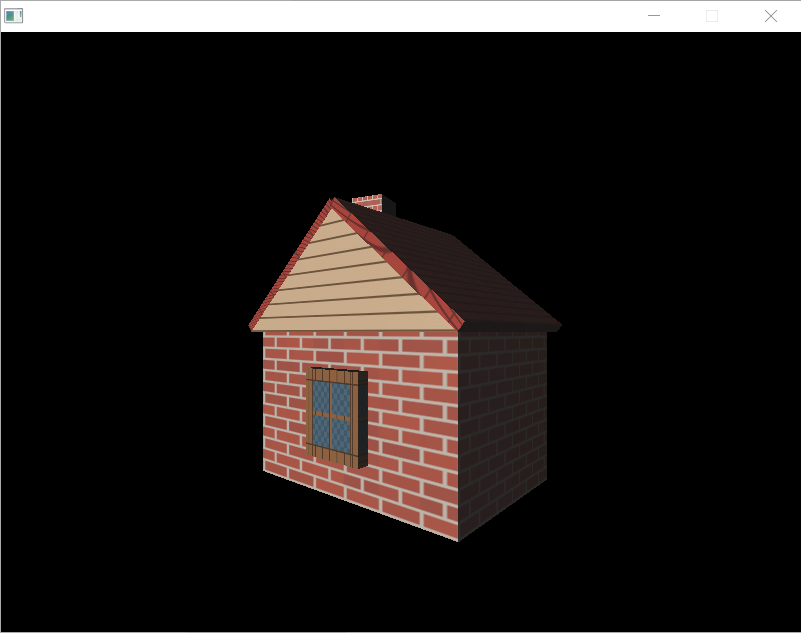
\includegraphics[width=0.65\textwidth]{images/house-frame.png}
		\caption {Пример кадра графического приложения}
	\end{figure}
	
	\note{
		Объекты в кадре:
		\begin{itemize}
			\item одна модель объекта
			\item один точечный свет
			\item одна камера
		\end{itemize}

		% В лекции про построение изображения сцена --- граф: несколько объектов, источников, камер.
		% Тип \texttt{Scene} в этой лабораторной --- параметры одного кадра, не граф.
		% Комментарий в \texttt{scene.hpp}: frame values for one model, not a scene graph.
		% После \texttt{processNode} у модели остаётся плоский список мешей.
		
	}
\end{frame}


\section{Модель}

\begin{frame}{Структура модели объекта}
	\begin{figure}
		\centering
		\resizebox{\textwidth}{!}{%
		\begin{tikzpicture}[
			font=\scriptsize,
			box/.style={
				draw,
				rounded corners=2pt,
				align=center,
				inner sep=2.5pt,
				minimum height=2.05em
			},
			>=stealth
		]
			\node[box] (model) at (0,0.4) {Model};
			\node[box] (meshes) at (2.35,1.55) {meshes};
			\node[box] (cache) at (2.35,-1.15) {textures\_loaded};
			\node[box] (mesh) at (4.7,1.55) {Mesh};
			\node[box] (verts) at (6.85,2.7) {vertices};
			\node[box] (idx) at (6.85,1.55) {indices};
			\node[box] (vao) at (6.85,0.4) {VAO};
			\node[box] (texs) at (6.85,-1.15) {textures};
			\node[box] (vert) at (8.85,2.7) {Vertex};
			\node[box] (pos) at (11.15,3.85) {Position};
			\node[box] (nrm) at (11.15,2.7) {Normal};
			\node[box] (tan) at (11.15,1.55) {Tangent};
			\node[box] (uv) at (11.15,0.4) {TexCoords};
			\node[box] (image) at (8.85,-2.3) {Texture};

			\draw[->] (model) -- (meshes);
			\draw[->] (model) -- (cache);
			\draw[->] (meshes) -- (mesh);
			\draw[->] (mesh) -- (verts);
			\draw[->] (mesh) -- (idx);
			\draw[->] (mesh) -- (vao);
			\draw[->] (mesh) -- (texs);
			\draw[->] (verts) -- (vert);
			\draw[->] (vert) -- (pos);
			\draw[->] (vert) -- (nrm);
			\draw[->] (vert) -- (uv);
			\draw[->] (vert) -- (tan);
			\draw[->] (cache) -- (image);
			\draw[->] (texs) -- (image);
		\end{tikzpicture}%
		}
		\caption{Иерархия полей модели}
	\end{figure}

	\note{
		{%\scriptsize
			Рассмотрим декомпозицию модели дома:
			\begin{itemize}
				\item \texttt{model}
				\begin{itemize}
					\item \texttt{house}
				\end{itemize}
				\item \texttt{meshes}
				\begin{itemize}
					\item \texttt{walls}, \texttt{roof\_L}, \texttt{roof\_R}
					\item \texttt{door}, \texttt{chimney}, \texttt{window}
				\end{itemize}
				\item \texttt{textures\_loaded}
				\begin{itemize}
					\item \texttt{wall.png}, \texttt{roof.png}
					\item \texttt{door.png}, \texttt{window.png}
				\end{itemize}
			\end{itemize}

			\scriptsize
			Примечание.
			\begin{itemize} \scriptsize
				\item model, meshes, texture links in *.gltf
				\item geometry (positions, normals, tangents, texcoords, indices) in *.bin
				\item textures in *.png
			\end{itemize}

			~
		}
	}
\end{frame}

\begin{frame}{}{}
	to be continued \dots
\end{frame}

\end{document}
